\documentclass[compress]{beamer}
\usepackage{ifthen,verbatim,ulem}

\newcommand{\isnote}{}
\xdefinecolor{lightyellow}{rgb}{1.,1.,0.25}
\xdefinecolor{darkblue}{rgb}{0.1,0.1,0.7}

%% Uncomment this to get annotations
%% \def\notes{\addtocounter{page}{-1}
%%            \renewcommand{\isnote}{*}
%% 	   \beamertemplateshadingbackground{lightyellow}{white}
%%            \begin{frame}
%%            \frametitle{Notes for the previous page (page \insertpagenumber)}
%%            \itemize}
%% \def\endnotes{\enditemize
%% 	      \end{frame}
%%               \beamertemplateshadingbackground{white}{white}
%%               \renewcommand{\isnote}{}}

%% Uncomment this to not get annotations
\def\notes{\comment}
\def\endnotes{\endcomment}

\setbeamertemplate{navigation symbols}{}
\setbeamertemplate{headline}{\mbox{ } \hfill
\begin{minipage}{5.5 cm}
\vspace{-0.75 cm} \small
\end{minipage} \hfill
\begin{minipage}{4.5 cm}
\vspace{-0.75 cm} \small
\begin{flushright}
\ifthenelse{\equal{\insertpagenumber}{1}}{}{Jim Pivarski \hspace{0.2 cm} \insertpagenumber\isnote/\pageref{numpages}}
\end{flushright}
\end{minipage}\mbox{\hspace{0.2 cm}}\includegraphics[height=1 cm]{../cmslogo} \hspace{0.1 cm} \includegraphics[height=1 cm]{../tamulogo} \hspace{0.01 cm} \vspace{-1.05 cm}}

\begin{document}
\begin{frame}
\vfill
\begin{center}
\textcolor{darkblue}{\Large Residual $\vec{B}$-field Errors}

\vfill
\begin{columns}
\column{0.3\linewidth}
\begin{center}
\large
\textcolor{darkblue}{Jim Pivarski}

\vspace{0.2 cm}
Alexei Safonov
\end{center}
\end{columns}

\begin{columns}
\column{0.3\linewidth}
\begin{center}
\scriptsize
{\it Texas A\&M University}
\end{center}
\end{columns}

\vfill
28 January, 2009

\end{center}
\end{frame}

%% \begin{notes}
%% \item This is the annotated version of my talk.
%% \item If you want the version that I am presenting, download the one
%% labeled ``slides'' on Indico (or just ignore these yellow pages).
%% \item The annotated version is provided for extra detail and a written
%% record of comments that I intend to make orally.
%% \item Yellow notes refer to the content on the {\it previous} page.
%% \item All other slides are identical for the two versions.
%% \end{notes}

\small

\begin{frame}
\frametitle{$\vec{B}$-field error cancellation method}
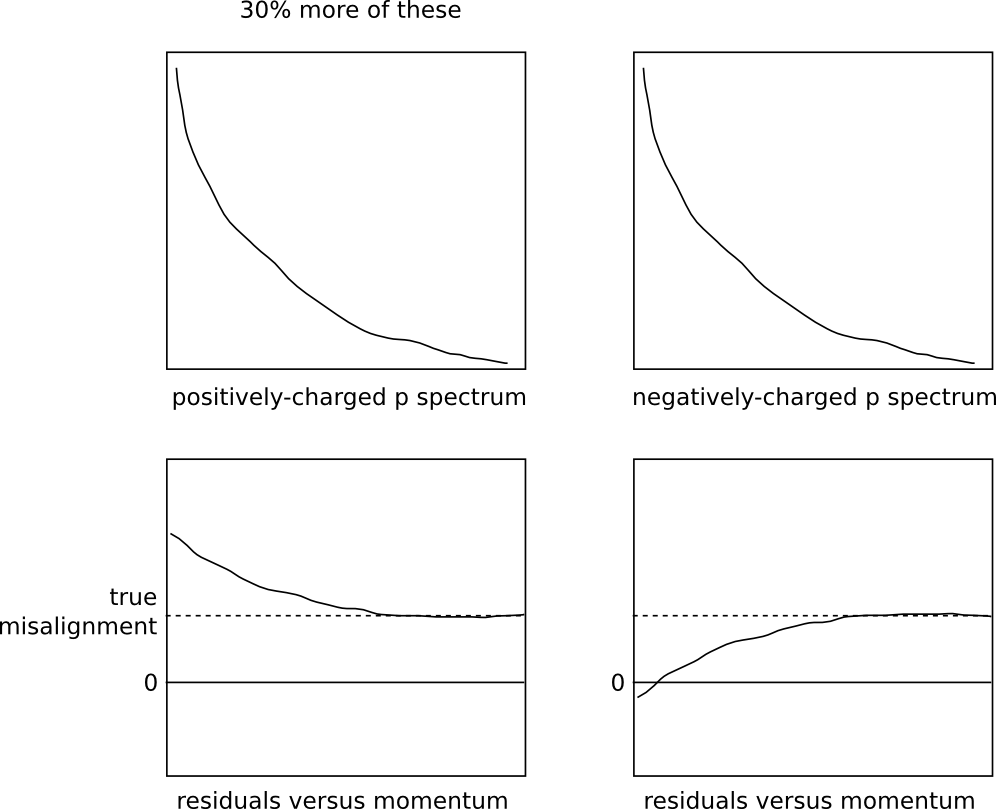
\includegraphics[width=0.7\linewidth]{bfield_explanation.png}

\begin{itemize}
\item Alignment measurement is the simple average of residuals in the positively-charged track bin and the negatively-charged track bin
\item Assumption: momentum spectra for the two charges is the same (also used by charge ratio analysis)
\end{itemize}
\end{frame}

\begin{frame}
\frametitle{An extreme case}
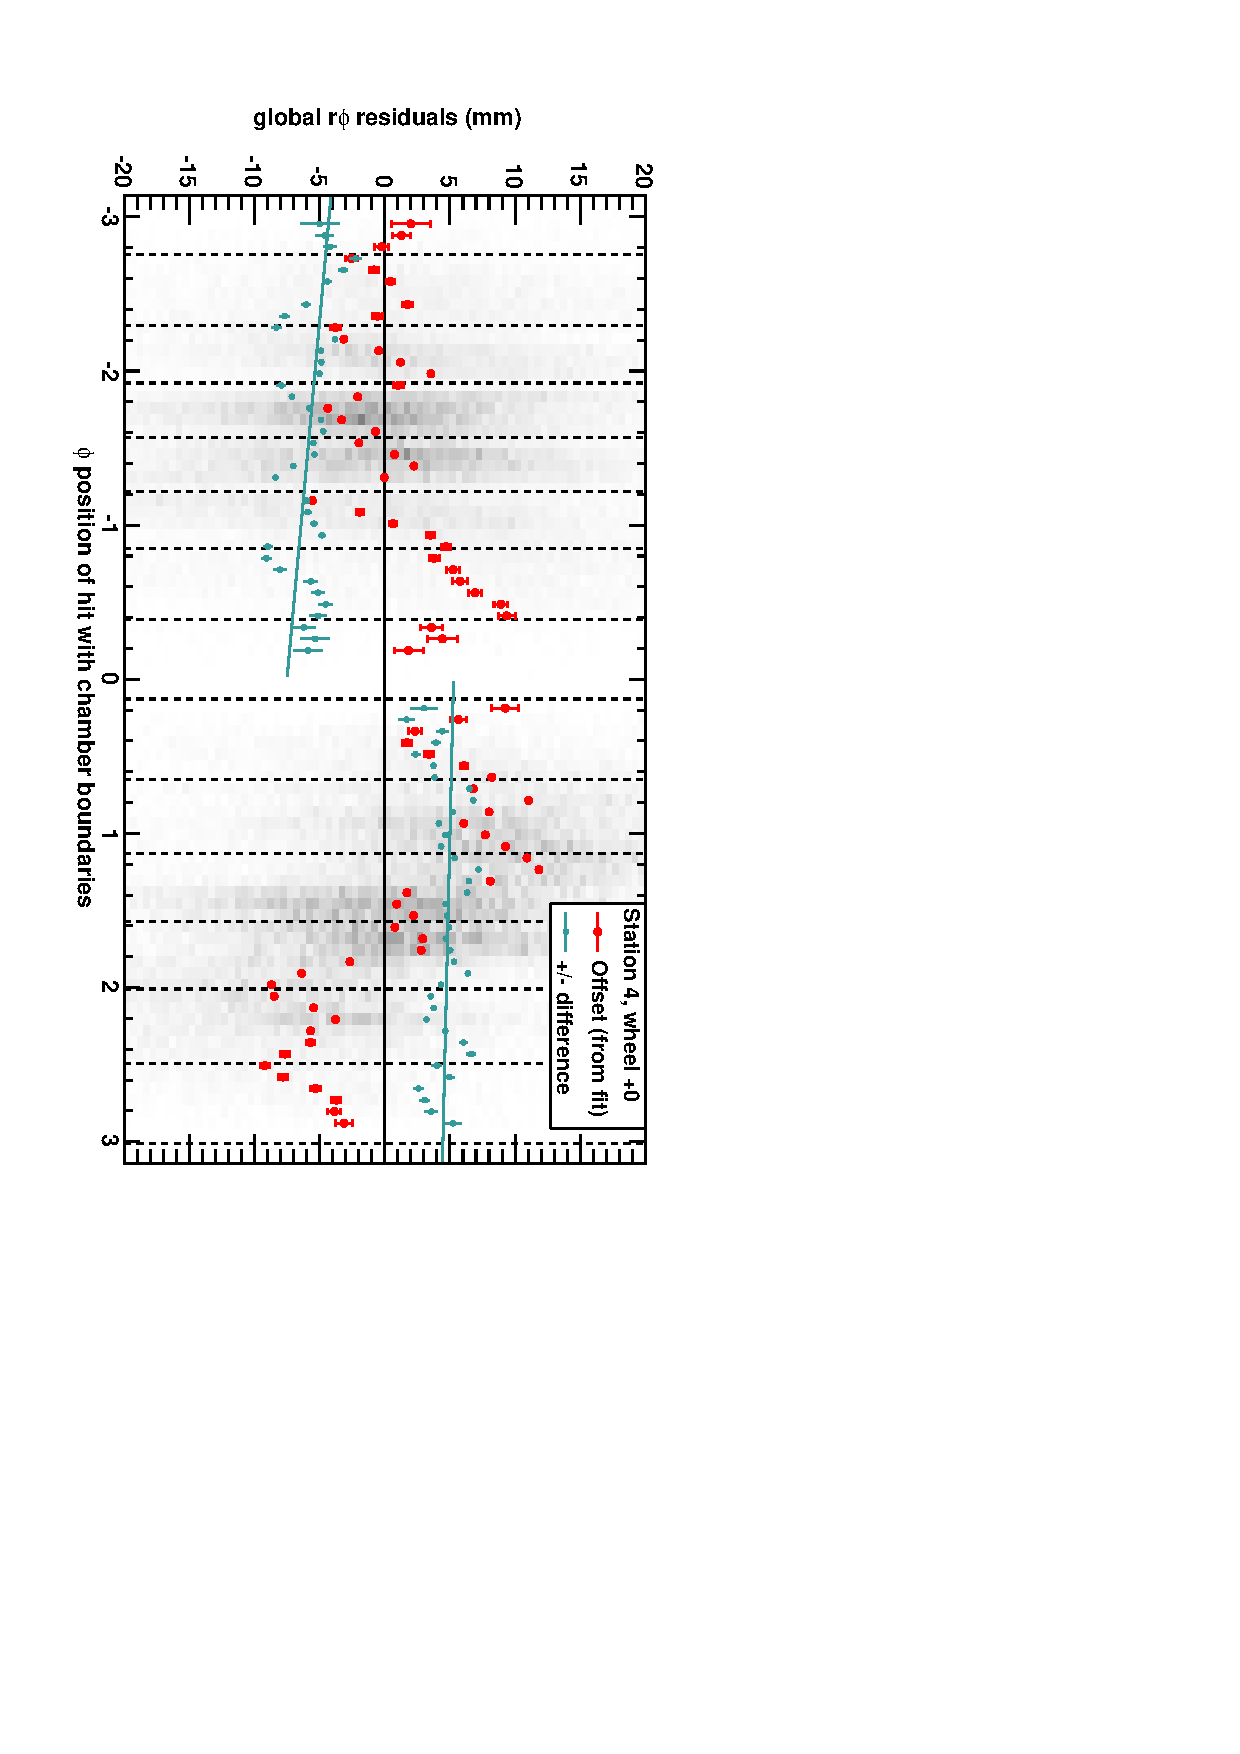
\includegraphics[height=0.5\linewidth, angle=90]{bfield_station4.pdf}

\begin{itemize}
\item Worst $\vec{B}$-field errors in station 4
\item Blue points are half the {\it difference} between the two bins; the error we would make if we used 100\% positive tracks and 0\% negative tracks
\item If we simply averaged all tracks, the systematic error would be 13\% of the blue points
\item The actual error is suppressed by the difference in 20~GeV momentum cut-off between the two charge signs, the fraction of charge misassignment, etc.
\item It's easily less than 1\% of the blue points (small enough to worry about other effects, first)
\end{itemize}

\label{numpages}
\end{frame}

\end{document}
